%!TEX root = ../sbc-template.tex

\emph{Deep Learning} (DL), também conhecido como Aprendizagem Profunda, compreende um conjunto de técnicas de ML que podem ser aplicadas em problemas de aprendizado supervisionado e não-supervisionado. A principal característica dos modelos neste domínio é a capacidade de representar e reconhecer características sucessivamente complexas, por meio da adição de níveis ou camadas de operações não lineares em sua arquiteturas, a exemplo das nas redes neurais profundas, máquinas de Boltzmann profundas e fórmulas proposicionais. Modelos deste tipo ganharam popularidade ao se mostraram capazes de resolver problemas complexos com um desempenho cada vez maior \cite{bengio2009learning}.

Há dois aspectos recorrentes nas diversas descrições de DL presentes hoje: (1) modelos que consistem de camadas ou estágios sucessivos de processamento de informações não-lineares; e (2) métodos para aprendizado supervisionado ou não-supervisionado de representação de características em camadas sucessivamente mais altas ou abstratas.

A melhoria do desempenho de modelos de DL é decorrente do aumento recente da quantidade de dados disponíveis sobre temas complexos, aliado com o aumento da disponibilidade de recursos computacionais para executar modelos mais robustos \cite{goodfellow2016deep}, \cite{deng2014deep}. Segundo a IBM, em 2017 foram gerados $2,5$ quintilhões de bytes de dados por dia, e 90\% do volume total de dados gerados até 2017 no mundo foi criado nos últimos dois anos \cite{ibm2017bigdata}.

Para exemplificar o efeito da adição de camadas aos modelos de DL, expõe-se na Figura \ref{fig:compara_redes} uma visão geral do aumento da profundidade de redes neurais convolucionais aplicadas à detecção de objetos em imagens. Nota-se que conforme são adicionadas camadas às redes, há uma diminuição no erro e, nas redes mais recentes, uma diminuição brusca do número de parâmetros a serem treinados. Isto indica que redes neurais convolucionais mais profundas tendem a capturar com maior precisão as características objetos em imagens, e que modelos mais modernos, a exemplo da GoogLeNet e ResNet, atingem este efeito enquanto diminuem a complexidade do problema ao derrubar o número de parâmetros a serem treinados.

\begin{figure}[!ht]
	\centering
	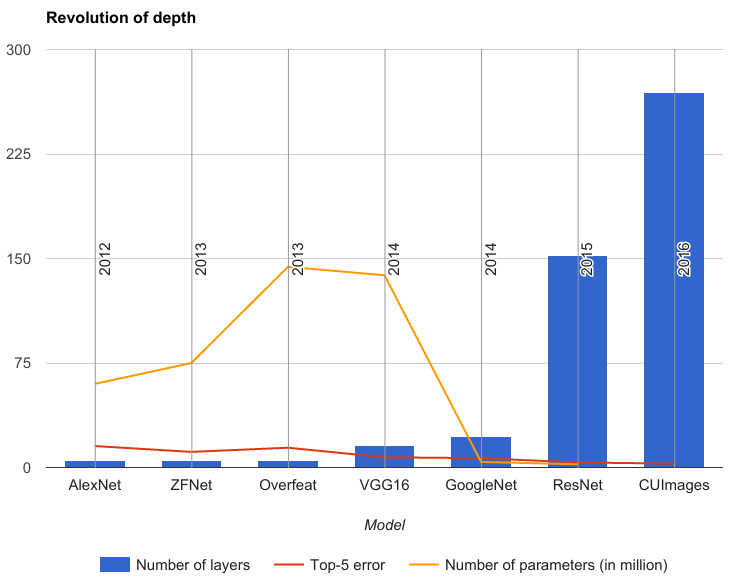
\includegraphics[width=0.8\textwidth]{img/compara_redes.png}
	\caption{Evolução de profunidade, taxa de erro e número de parâmetros de redes neurais convolucionais com o passar dos anos. Fonte: \cite{mediumcnn}.}
	\label{fig:compara_redes}
\end{figure}

\subsubsection{Breve Histórico}

Historicamente, o conceito de DL se originou de pesquisas sobre Redes Neurais Artificiais (RNA), mais especificamente, as redes neurais \emph{feed-forward} com muitas camadas ocultas, também chamadas de redes neurais profundas \cite{deng2014deep}. O termo \emph{deep learning} foi utilizado pela primeira vez em \cite{dechter1986learning}, no contexto da descoberta de todas as configurações de conflitos mínimas no fim de um problema de satisfação de limitação (em inglês, \emph{Constraint-Satisfaction Problem -- CSP}). Em ANO, foi utilizado para designar métodos que têm a ver com o DL moderno em PUBLICAÇÃO, que trata de TEMA. A partir daí, o termo passou a designar modelos compostos de várias camadas sucessivas de operações não lineares utilizados para o aprendizado de determinada tarefa.

A história da pesquisa sobre este DL está dividida em três ondas, ou gerações. A primeira geração foi marcada pelo desenvolvimento de modelos lineares simples, compostos apenas por um neurônio, como o modelo de \cite{mcculloch1943logical} e o Perceptron de \cite{rosenblatt1958perceptron}. A segunda onda, iniciada nos anos 1980, teve como idéia central a inteconexão entre vários neurônios \cite{rumelhart1986parallel}, além do algoritmo de \emph{back-propagation} \cite{rumelhart1986backpropagation}. No final da segunda era, \cite{hochreiter1997long} propuseram o modelo \emph{long short-term memory} (LSTM) e \cite{lenet} propuseram a LeNet \todo[inline]{EXPLICAR IMPORTÂNCIA DA LENET}. A teceira onda começa em 2006 com a publicação do artigo \cite{hinton2006fast}, que apresenta as \emph{deep belief networks}, um tipo de RNA que  \todo[inline]{EXPLICAR}. Foi nesta onda, que dura até o presente momento \cite{goodfellow2016deep}, que o termo \emph{deep learning} se popularizou. Na conjectura atual, redes neurais profundas têm superado sistemas que aplicam ML e funcionalidades desenhadas à mão em competições envolvendo inteligência artificial.

\begin{figure}[!h]
	\centering
	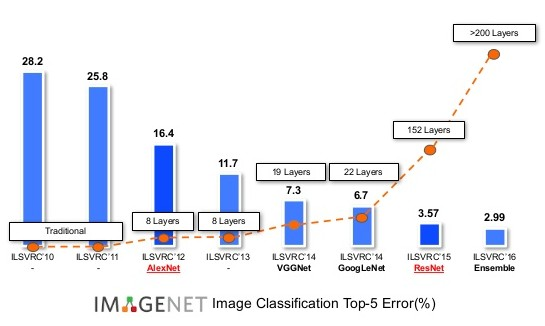
\includegraphics[width=0.8\textwidth]{img/compara_redes_ilsvrc.png}
	\caption{Evolução do erro dos modelos vencedores da competição ILSVRC pela profundidade das redes neurais \cite{dl_ILSVRC}}
	\label{fig:compara_redes_ilsvrc}
\end{figure}

A \emph{ImageNet Large Scale Visual Recognition Challenge}, ou ILSVRC, é uma competição em que times de pesquisa avaliam seus algoritmos em um conjunto de dados fornecido, e competem para chegar à melhor acurácia em várias tarefas de reconhecimento visual. Em 2011, uma boa classificação no ILSVRC tinha por volta de $25\%$ de erro. Em 2012, uma RNA convoluncional chamada AlexNet atingiu $16.4\%$ de erro. No gráfico da Figura \ref{fig:compara_redes}, que mostra os melhores colocados na competição da ImageNet ano a ano, nota-se a diferença entre o erro atingido pelo modelo do ano anterior, que consiste de DETALHAR MODELO DE 2011, para a AlexNet. \todo[inline]{EXPLORAR MAIS A IMAGEM.}

Apesar de ter tido um foco inicial em técnicas novas de aprendizado não-supervisionado e na habilidade de modelos profundos de boa generalização a partir de conjuntos de dados pequenos, o momento atual das pesquisas em DL envolvem o uso de técnicas de aprendizado supervisionado bem mais antigas para o \emph{leverage} de conjuntos de dados massivos e categorizados. Um exemplo destas técnicas são as redes neurais convolucionais com múltiplas camadas, que impulsionaram os avanços recentes alcançados no campo da visão computacional. Na Seção \ref{subsubsec:rnc} a seguir, serão definidas as redes neurais convolucionais, suas características e particularidades. Na Seção \ref{subsubsec:modelos_canonicos} serão tratadas algumas das redes neurais convolucionais profundas que ganharam destaque em competições como o ILSVRC responsáveis pela fama atingida nos últimos anos.


\subsubsection{Redes Neurais Convolucionais} \label{subsubsec:rnc}
Redes neurais convolucionais (CNN, do inglês, \emph{Convolutional Neural Networks}) são uma classe de redes neurais \emph{feed-forward} que têm se mostrado bem-sucedidas no processamento de dados que têm uma topologia bem definida e estruturada em uma grade, a exemplo de séries temporais e imagens. Sua principal característica envolve o uso de convoluções no lugar de multiplicações de matrizes em ao menos uma das camadas da rede neural \cite{goodfellow2016deep}. Este modelo pode ser aplicado em tarefas de classificação, regresssão, localização, detecção, entre outros.

Cada camada das redes neurais convolucionais é composta por uma etapa de convolução, seguida por uma ativação não-linear, finalizando em \emph{pooling}, como mostra a Figura \ref{fig:cnn_camada}. A seguir, serão explanadas cada uma destas etapas.

\begin{figure}
	\centering
	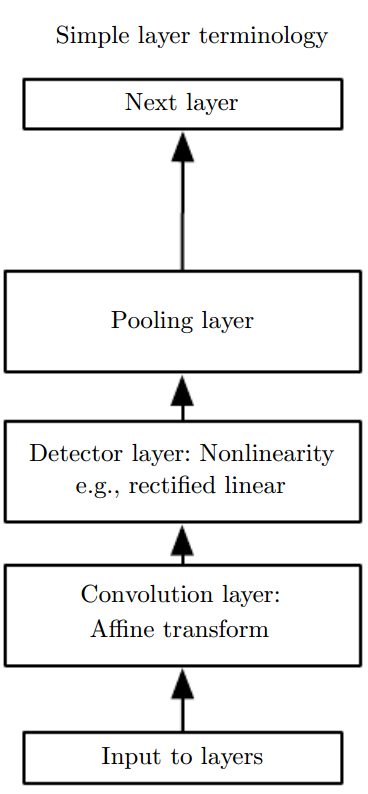
\includegraphics[height=0.3\textheight]{img/cnn_camada.png}
	\caption{Componentes de uma camada de uma rede neural convolucional \cite{goodfellow2016deep}. }
	\label{fig:cnn_camada}
\end{figure}


\paragraph{Convolução}
\ \ \newline
A operação de convolução descreve a média ponderada de uma determinada função $x_1(t)$ sob um intervalo fixo de uma variável, enquanto os pesos da média ponderada considerada pertencem à função $x_2(t)$ amostrados em intervalos $a$ \cite{bracewell1986fourier}. Assim, a convolução $s(t)$ de duas funções $x_1(t)$ e $x_2(t)$ é uma função $f: \mathds{Z} \rightarrow \mathds{R}$ representada simbolicamente por $x_1(t) * x_2(t)$ e definida de acordo com a Equação \ref{eq:int_convolucao} \cite{lathi2006sinais}.
\begin{equation}\label{eq:int_convolucao}
	s(t) = x_1(t) * x_2(t) = \int_{-\infty}^{\infty} x_1(a) x_2(t-a)da
\end{equation}

Quando a operação de convolução é aplicada em aprendizagem de máquina, a primeira função $x_1(t)$ é chamada de \emph{input}, a segunda função $x_2(t)$ é chamada de \emph{kernel}, e a saída $s(t)$ é chamada de mapa de \emph{feature map}, ou mapa de características. Neste caso, a entrada normalmente é um vetor multidimensional de dados e o núcleo é um vetor multidimensional de pesos que devem ser adaptados pelo algoritmo de aprendizado de máquina. Em redes neurais convolucionais, os vetores multidimensionais de entrada e núcleo são chamados tensores. Além disto, assume-se que os valores dos tensores são zero em todos os pontos menos os que estão guardados em memória, ou seja, a operação de convolução é implementada apenas nas posições declaradas dos vetores de dados e peso. Assim, para uma imagem bidimensional de tamanho $(m,n)$ $I$ como entrada, tem-se um núcleo bidimensional $K$, e a operação de convolução é definida como exemplificado na Equação \ref{eq:conv_img}, para cada posição $(i,j)$ do mapa de características resultante \cite{goodfellow2016deep}.

\begin{equation}\label{eq:conv_img}
	S(i,j) = I(i,j)*K(i,j) = \sum_{m}\sum_{n}I(m,n)K(i-m,j-n)
\end{equation}

A convolução é comutativa, ou seja, as Equações \ref{eq:conv_img_eq} e \ref{eq:conv_img} são equivalentes, salvo que no primeiro caso há a convolução da imagem pelo núcleo, enquanto no segundo há a convolução do núcleo pela imagem. Comumente, a Equação \ref{eq:conv_img} é a implementada em algoritmos de redes neurais convolucionais, haja visto que existem menor variação no intervalo de valores válidos de $m$ e $n$, o que diminui o custo computacional.

\begin{equation}\label{eq:conv_img_eq}
	S(i,j) = K(i,j)*I(i,j) = \sum_{m}\sum_{n}I(i-m,j-n)K(m,n)
\end{equation}

A propriedade comutativa surge graças à ação de revolver o núcleo em relação à imagem, e não tem aplicação prática. Porém, esta propriedade não tem fins práticos além da prova da operação de convolução. Assim, é comum que seja implementada correlação cruzada, indicada na Equação \ref{eq:correlacao_img_eq}, semelhante à convolução dada na Equação \ref{eq:conv_img_eq} sem que haja o espelhamento do núcleo em relação à imagem.

\begin{equation}\label{eq:correlacao_img_eq}
	S(i,j) = I(i,j)*K(i,j) = \sum_{m}\sum_{n}I(i+m,j+n)K(m,n)
\end{equation}

\paragraph{Ativação}
\ \ \newline

\paragraph{Pooling}
\ \ \newline
Depois de realizar várias operações de convolução em paralelo para gerar um conjunto de ativações lineares e alimentá-las a funções de ativação não-lineares, como \emph{ReLU}, \emph{Softmax}, etc, na chamada etapa de detecção, chega-se à etapa de \emph{pooling}. Uma função de \emph{pooling} substitui a saída da rede em determinada localização por uma síntese estatística das saídas vizinhas. Por exemplo, a função \emph{max pooling} retorna o valor máximo em uma área retangular, enquanto a \emph{average pooling} retorna a média das saídas de um retângulo. %O objetivo destas funções é fazer com que


\subsubsection{Modelos Canônicos de Redes Neurais Convolucionais para Detecção de Objetos em Imagens} \label{subsubsec:modelos_canonicos}
